\section{Theory and Concepts}

\textbf{Federated Learning Architecture:} The platform follows a coordinator-client model where a central server orchestrates training rounds while hospitals maintain complete data sovereignty. During each round, the coordinator broadcasts the global model to participating clients, who perform local training on private datasets and transmit only encrypted model updates back. The coordinator aggregates these updates using weighted averaging or advanced techniques, producing an improved global model redistributed for the next round. This fundamentally differs from centralized learning by keeping sensitive patient data local, satisfying privacy regulations while enabling collaborative AI development.

\textbf{Aggregation Algorithms:} The platform implements multiple aggregation strategies. FedAvg serves as the baseline using weighted averaging:
\[ w_{global}(t+1) = \sum(n_k / N) \times w_k(t+1) \]
where each hospital's contribution is weighted by dataset size. FedOpt extends this by applying adaptive optimization (Adam, Adagrad) at server level:
\[ w_{global}(t+1) = w_{global}(t) - \eta \times Optimizer(\Delta w_{aggregated}) \]
maintaining momentum terms that smooth inconsistent updates from heterogeneous client datasets. FedMA uses Hungarian algorithm for neuron matching before averaging, achieving higher quality but with 30-50\% overhead. FedProx adds a proximal term enabling partial work from resource-constrained clients.

\textbf{Performance-Aware Weighted Aggregation (PAWA):} Our novel algorithm dynamically computes client weights based on four factors:
\begin{enumerate}
    \item \textbf{Performance Score (40\% weight)} combining validation accuracy and inverse loss:
    \[ \frac{accuracy + \left( \frac{1}{1 + loss} \right)}{2} \]
    \item \textbf{Dataset Size Score (30\% weight)} normalized by total examples:
    \[ \frac{client\_examples}{total\_examples} \]
    \item \textbf{Data Quality Score (20\% weight)} tracking loss improvement consistency over 3 rounds.
    \item \textbf{Progress Score (10\% weight)} measuring recent improvement:
    \[ \frac{previous\_loss - current\_loss}{previous\_loss} \]
\end{enumerate}
Each factor is normalized to [0,1], combined with configurable weights, and clients below performance threshold (default 0.3) are penalized (weight $\times$ 0.1). Final weights use temperature-scaled softmax (default temperature=2.0) for smooth distribution, effectively handling non-IID medical data by prioritizing high-performing, consistent clients.

\textbf{Non-IID Data Challenges:} Medical imaging exhibits severe heterogeneity from demographic variations, equipment differences (scanner manufacturers, protocols), disease prevalence variations, and institutional specializations. These cause weight divergence where local models learn conflicting features. The platform addresses this through PAWA's performance-based weighting, adaptive learning rates in FedOpt, data quality monitoring, and convergence-based dynamic adjustment.

\textbf{Deep Learning Architecture:} The platform uses ResNet-50, a 50-layer residual network employing skip connections that mitigate vanishing gradients in deep networks. Transfer learning leverages ImageNet pretrained weights, adapting general visual features (edges, textures, shapes) to medical domains, significantly reducing training time compared to training from scratch.

\textbf{Core Technologies:} PyTorch provides dynamic computational graphs, automatic differentiation via backpropagation, and GPU acceleration through CUDA. Flower (v1.5) orchestrates federated training with Strategy interface for implementing custom aggregation algorithms, supporting synchronous and asynchronous modes, client sampling, and built-in FedAvg/FedAdam implementations. FastAPI builds the coordinator backend with async/await for concurrent handling, automatic OpenAPI documentation, Pydantic validation, and WebSocket support for real-time monitoring. Next.js 15 powers hospital dashboards with server-side rendering, file-based routing, and React hooks for state management. Docker ensures consistent deployment through containerization, packaging applications with all dependencies into portable images. Supabase provides PostgreSQL database with real-time subscriptions, auto-generated RESTful APIs, row-level security, and JSONB columns for flexible metadata storage.

\textbf{Security Infrastructure:} HTTPS/TLS encrypts communications using RSA 2048-bit key exchange and AES-256-GCM data transmission. Role-based access control (RBAC) restricts functionality through JWT authentication with signed tokens carrying user identity and permissions. WebSocket enables full-duplex communication over persistent connections for real-time monitoring dashboards, reducing latency compared to HTTP polling.

\section{Dataset Description}

\textbf{TB Chest X-ray Dataset:} Contains 7,000 chest X-ray images (Normal vs. TB positive) from NIH database, 512$\times$512 to 1024$\times$1024 grayscale resolution. Distributed across 4 hospitals with non-IID characteristics: Hospital 1 (1,750 images, 25\%, higher TB prevalence), Hospital 2 (1,400 images, 20\%, balanced), Hospital 3 (2,100 images, 30\%, pediatric focus), Hospital 4 (1,750 images, 25\%, geriatric focus).

\textbf{Diabetic Retinopathy Dataset:} Contains 3,662 retinal fundus photographs (5 severity levels: 0-4) from screening programs, 2048$\times$1536 color images. Distribution: Hospital 1 (916 images, 25\%, severe cases), Hospital 2 (732 images, 20\%, screening population), Hospital 3 (1,098 images, 30\%, balanced), Hospital 4 (916 images, 25\%, moderate cases).

\textbf{Brain Tumor MRI Dataset:} Contains 3,624 brain MRI scans (Glioma, Meningioma, Pituitary, No tumor) as T1-weighted contrast-enhanced images, 512$\times$512 grayscale. Distribution: Hospital 1 (906 images, 25\%, glioma specialization), Hospital 2 (724 images, 20\%, balanced), Hospital 3 (1,087 images, 30\%, meningioma focus), Hospital 4 (907 images, 25%, general cases).

\textbf{Data Characteristics:} All datasets exhibit significant non-IID properties including class imbalance, domain shift from different equipment, demographic variations, and quality variations from scanner resolution differences. Total 14,286 images distributed across 4 hospitals with each maintaining 1,000-2,800 images locally—sufficient for meaningful training while benefiting from collaboration.

\section{Design and Methodology}

\textbf{System Design Principles:}
\begin{enumerate}
    \item \textbf{Privacy-first architecture:} No raw data transmission across the network.
    \item \textbf{Modularity:} For independent component development and easier maintenance.
    \item \textbf{Scalability:} Supporting dynamic hospital addition up to 4 nodes.
    \item \textbf{Production-readiness:} Comprehensive error handling and audit logging.
    \item \textbf{Usability:} Intuitive interfaces designed for non-technical staff.
\end{enumerate}

\textbf{Federated Learning Workflow:} Training proceeds iteratively through five phases:

\begin{enumerate}
    \item \textit{Initialization:} Coordinator initializes ResNet-50 with ImageNet pretrained weights, stores in Supabase, broadcasts parameters to registered hospitals via secure channels.
    \item \textit{Local Training:} Each hospital receives global model, loads local medical imaging data, trains for 5-10 epochs using PyTorch, computes weight updates (new\_weights - old\_weights), encrypts updates for transmission.
    \item \textit{Aggregation:} Coordinator collects encrypted updates, decrypts and validates (checking shapes, detecting NaN), applies selected algorithm (FedAvg, FedOpt, FedMA, FedProx, or PAWA), weighs updates appropriately, generates improved global model, stores new version in database. For PAWA, the coordinator computes performance scores from each client's validation metrics, combines with dataset sizes and quality trends, applies temperature-scaled softmax with threshold filtering, and performs weighted averaging using computed weights.
    \item \textit{Distribution:} Coordinator broadcasts updated global model to all hospitals, sends convergence metrics via WebSocket to monitoring dashboards.
    \item \textit{Convergence Check:} System evaluates if target accuracy (95\% centralized baseline) achieved or maximum rounds completed, continuing if needed or finalizing and exporting trained model if complete.
\end{enumerate}

\textbf{Preprocessing Pipeline:} Standardized across hospitals:
\begin{enumerate}
    \item Load images using Pillow supporting JPEG, PNG, and DICOM formats.
    \item Resize to $224 \times 224$ using bicubic interpolation.
    \item Normalize to $[0,1]$ and apply ImageNet statistics ($mean=[0.485, 0.456, 0.406], std=[0.229, 0.224, 0.225]$).
    \item Strip EXIF metadata and text overlays for privacy.
    \item Apply augmentation ($\pm15^\circ$ rotations, horizontal flips, $\pm20\%$ brightness/contrast, random crops).
    \item Validate quality (detect corruption, check distributions, ensure minimum resolution).
\end{enumerate}

\textbf{Communication Protocol:} Two channels implemented:
\begin{enumerate}
    \item \textbf{REST API via FastAPI:} POST \texttt{/api/submit\_update} for model uploads, GET \texttt{/api/get\_model} for retrieving global model, JWT authentication in Authorization headers, and JSON payloads with Base64-encoded tensors.
    \item \textbf{WebSocket at \texttt{wss://coordinator/ws}:} For persistent connections, real-time progress broadcasts (accuracy, loss, round number), client status updates, and bidirectional heartbeat monitoring.
\end{enumerate}

\textbf{Security Implementation:} Multi-layered protection includes TLS 1.3 encryption with certificate pinning, JWT tokens with 24-hour expiration and refresh rotation, bcrypt password hashing, RBAC enforcing least privilege, and immutable audit logs of all model transmissions with automatic alerting for suspicious patterns.

\textbf{Monitoring and Observability:} Real-time monitoring provides: Training Metrics (global accuracy/loss per round, per-client training time, convergence rate, communication overhead), System Health (client connectivity, GPU utilization, network latency, error rates), Dashboard Features (live charts updated via WebSocket, client status tables, round progress indicators, performance degradation alerts). For PAWA, dashboards additionally display per-client weight evolution across rounds, factor contribution breakdown, and performance threshold violations.

\section{System Architecture}

\textbf{Three-Tier Architecture:}

\textit{Tier 1 - Hospital Clients:} Next.js web applications with Docker containers housing PyTorch training environment, local storage for medical datasets, WebSocket clients for real-time coordinator communication.

\textit{Tier 2 - Coordinator Server:} FastAPI application on Vercel cloud platform, Flower server orchestrating federated rounds with PAWA aggregation engine, WebSocket server broadcasting training updates, multi-algorithm aggregation engine (FedAvg, FedOpt, FedMA, FedProx, PAWA).

\textit{Tier 3 - Data Layer:} Supabase PostgreSQL for model versioning and metadata, audit log storage for compliance, user authentication and role management, real-time subscriptions for live dashboard updates.

\textbf{Component Interactions:}
\begin{enumerate}
    \item \textbf{Client Registration:} Via authenticated WebSocket providing institution ID and dataset metadata.
    \item \textbf{Training Initiation:} Broadcasting initial ResNet-50 model and configuration including PAWA parameters.
    \item \textbf{Local Training:} At each hospital using PyTorch on private images.
    \item \textbf{Update Submission:} With encrypted uploads via HTTPS POST including validation metrics for PAWA.
    \item \textbf{Aggregation:} Collecting updates, computing PAWA weights from performance, size, quality, and progress scores, applying weighted averaging, and storing the new model in Supabase.
    \item \textbf{Distribution:} Pushing updated global model via WebSocket/REST with computed weight justifications.
    \item \textbf{Monitoring:} Broadcasting real-time metrics and PAWA weight distributions to Next.js dashboards.
\end{enumerate}

\textbf{Scalability Design:} Vercel serverless functions auto-scale based on request volume, WebSocket connections distributed across instances, Supabase handles 100,000+ concurrent connections. Docker containers enable identical deployment across unlimited hospitals, Flower supports 100+ clients, asynchronous aggregation allows subset participation. PostgreSQL partitioning for large audit logs, JSONB indexes for fast metadata queries, automated archival of old model versions.

\begin{figure}[H]
    \centering
    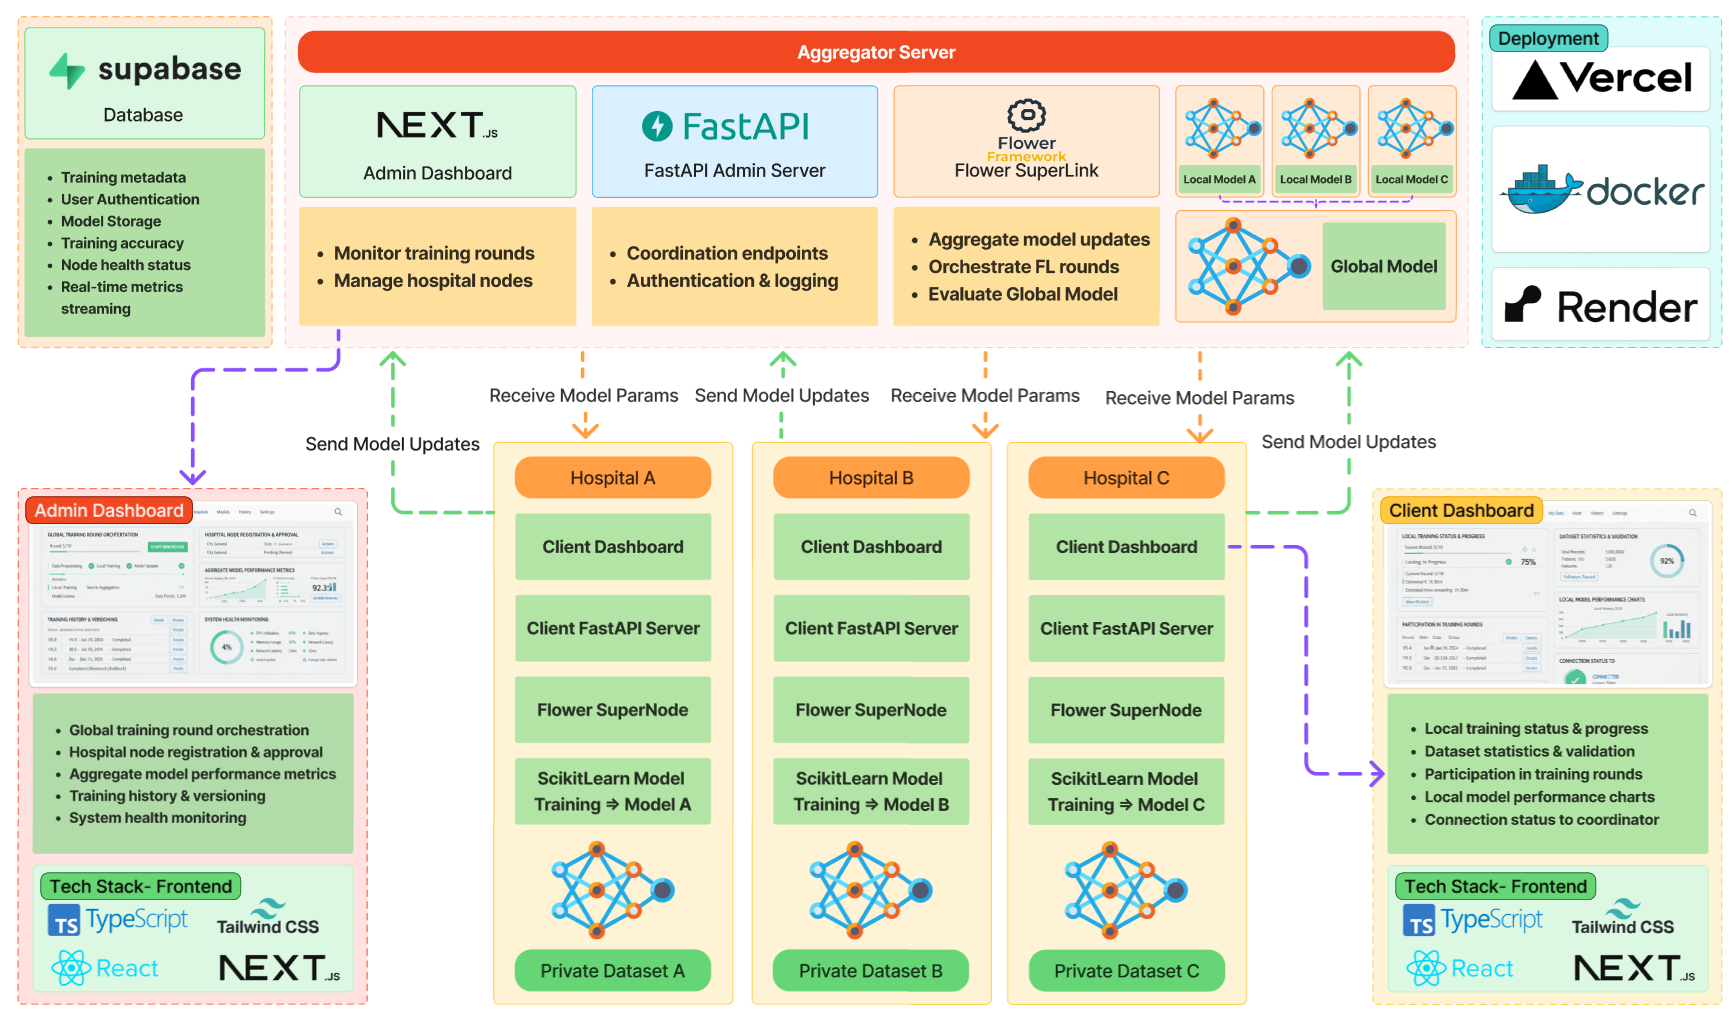
\includegraphics[width=0.9\textwidth]{images/fedml-architecture.png}
    \caption{Federated Learning System Architecture}
    \label{fig:fedml_architecture}
\end{figure}

\section{Tools and APIs}

\textbf{Core Frameworks:} Flower v1.5 for federated orchestration with custom PAWA Strategy class, PyTorch v2.0 for deep learning with GPU support, FastAPI v0.104 for async web framework, Next.js 15 for React-based frontend, Docker v24.0 for containerization.

\textbf{Data Processing:} NumPy v1.24+ for numerical operations, Pillow v10.0+ for image processing, torchvision v0.15+ for pretrained ResNet-50 and augmentation, pandas for metrics logging.

\textbf{Database and Storage:} Supabase providing PostgreSQL v14+ with real-time subscriptions and RESTful APIs, storing model versions, audit logs, PAWA weight histories, and performance metrics.

\textbf{Deployment:} Vercel for serverless FastAPI coordinator and Next.js dashboards, Render for alternative backend hosting, Docker Hub for client application distribution, Let's Encrypt for free SSL/TLS certificates.

\textbf{Key APIs:} Flower API with \texttt{start\_server()}, \texttt{start\_client()}, custom \texttt{PAWAStrategy} class overriding \texttt{aggregate\_fit()} with performance-aware weight computation; FastAPI endpoints for model submission and retrieval; Supabase REST API for automatic database CRUD; External resources including Kaggle datasets and ImageNet weights from PyTorch model zoo.

\textbf{Security Tools:} pyjwt for token generation, jsonwebtoken for validation, bcrypt for password hashing, TLS 1.3 for transport encryption.

\section{Summary}

The system combines federated learning theory with modern web technologies for production-ready healthcare AI. Core concepts include FedAvg baseline aggregation, FedOpt adaptive optimization, and novel PAWA algorithm dynamically weighting clients based on performance (40\%), dataset size (30\%), data quality (20\%), and progress (10\%) using temperature-scaled softmax with threshold filtering. ResNet-50 CNNs with ImageNet transfer learning classify medical images across three datasets: TB Chest X-rays (7,000 images), Diabetic Retinopathy (3,662 images), Brain Tumor MRI (3,624 images), distributed across 4 hospitals with realistic non-IID characteristics.

The three-tier architecture separates hospital clients (Docker containers with PyTorch), coordinator server (Flower + FastAPI orchestrating PAWA aggregation), and data layer (Supabase for models and audit logs). Communication uses HTTPS REST for model transmissions and WebSocket for real-time monitoring, secured with TLS encryption and JWT authentication. The methodology implements iterative rounds where hospitals train locally for 5-10 epochs, submit encrypted updates with validation metrics, and coordinator aggregates using PAWA's multi-factor weighting, adapting to client performance trends.

Standardized preprocessing ensures consistency: 224$\times$224 resizing, ImageNet normalization, privacy-preserving metadata stripping, and augmentation. The technology stack—Flower for orchestration, PyTorch for training, FastAPI for backend, Next.js for dashboards, Docker for deployment, Supabase for persistence—provides a scalable, secure platform. PAWA's adaptive weighting effectively handles medical data heterogeneity by prioritizing high-performing, consistent clients while maintaining fairness through temperature-scaled softmax, addressing critical gaps in healthcare AI collaboration.

